\chapter{Detailed System Design}

\section{Operator}
\todo{Describe Operator or drop this section.}

\section{Core Modules}

\subsection{Module Initialization}

The initialization of each core module follows the procedure that is 
described in detail in chapter \textit{System Initialization} in the BCI2000 
Project Outline: 

Each module publishes its requests for parameters and states to 
the Operator module, which configures those and sends them back.
After Data Acquisition received all parameters and states, it tries to connect
to Signal Processing and -- upon successful connection -- sends a positive status 
message to the Operator.
In the same way, Signal Processing connects to the Application and the
Application module connects to the Data Acquisition module.
After the Operator received status messages from all three core modules, the 
system is fully initialized and is triggered to start, as soon as the Operator 
sends the state \textit{Running} with a value of 1 to the Data Acquisition.

\subsection{System Termination}

To each of the three core modules, the operator module indicates system termination
by closing the connection to that module.

When a core module loses connection to the two other core modules it is connected
to, it will send an error message to the operator, and then quit.
The operator module, in turn, will close the connections to the remaining core
modules.


\section{EEG Data Acquisition}
\label{sec:sourcedescription}
The EEG Data Acquisition (or Source) module's role is to wait for data blocks
coming in from the A/D hardware, and to send these blocks of data on to Signal
Processing, thus acting as the on-line system's ``metronome" synchronized to 
the A/D hardware clock.
At the same time, it receives state vector information from the Application 
module, and saves this state vector information to a file in BCI2000 .dat
format, together with the raw digitized data.

During normal operation (\textit{Running} is 1), the EEG source module 
runs in a data acquisition loop that basically reads
\begin{verbatim}
1: While Running
2:   Save state vector to file
3:   Wait for A/D data
4:   Send A/D data to Signal Processing
5:   Wait for state vector from Application
6:   Save A/D data to file
\end{verbatim}

Note that statement 3 as well as statement 5 are blocking operations, i.e.\ 
the module will wait for A/D data as well as for the state vector data
coming in from the Application module.

This mode of operation requires a sufficiently fast system to work properly.
For our purposes, a ``fast" system is a system where 
\begin{itemize}
\item synchronous I/O operations (2, 4, 5, and 6) require an execution time
      that is small compared to the duration of a data block
      (as given by the sampling rate and the sample block size), and
\item the time required by the Signal Processing and Application modules
      for processing the data sent out in statement 4 is small compared
      to the duration of a data block.
\end{itemize}
In an on-line system, the time between sampling of a data block, and display
of the resulting feedback information to the subject, is critical.
Given a ``sufficiently fast" system as defined above, only statement 4 will enter
into this critical time path, while the time spent on execution of the remaining
statements will reduce the waiting interval occurring in statement 3.


\newpage
\section{Signal Processing}

\subsection{Overview}

Signal Processing acts like a black box to the rest of the system -- it receives 
EEG signals from the Data Acquisition and sends control signals on to the 
Application. Figure \ref{sigprocdataflow} illustrates the data flow in this 
implementation. As layed out in Figure \ref{sigprocdataflow}, there are basically 
5 main filters (Calibration, Spatial Filter, Temporal Filter, Classifier, and 
Normalizer) and 6 different signals (A (EEG signal), B, C, D, E, F 
(control signal)). The dimensionality 
of each of these signals is described in their respective filter description. 

\begin{figure}[ht]
 \centerline{\scalebox{0.8}{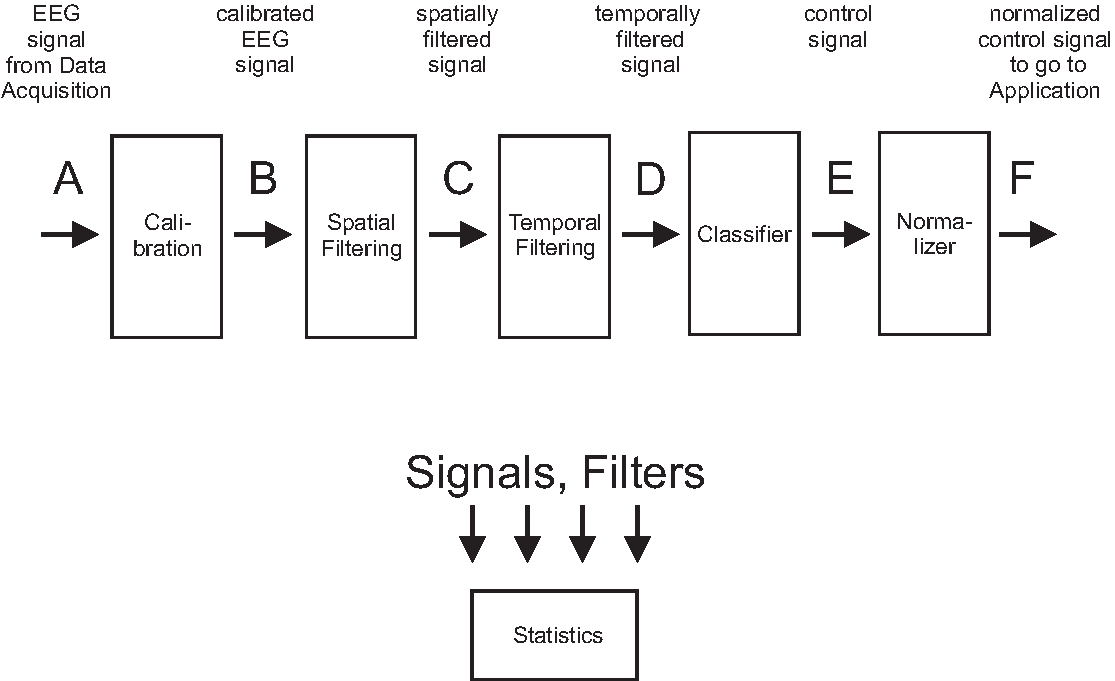
\includegraphics{figures/SigProcDataFlow}}}
 \caption{Data flow in the signal processing module}
 \todo{In the actual implementation, the Statistics filter is a pass-through
       filter for signal E (position), and communicates with the normal filter
       by changing parameters(arrow direction). However, the diagram
       might be called roughly correct in a more abstract sense.}
 \label{sigprocdataflow}
\end{figure}

\subsection{Goals}

As described in chapter \ref{des_consid_goals}, one of the goals for this system 
is for each module to be as independent of the others as possible, e.g., Signal 
Processing should not have to take the type of data collection hardware into 
account. For the same reason, Application should (ideally) not have to know 
about the used signal processing method. While in real-world situations this 
will not be possible, control signals shall be normalized to the value range of 
short integers (-32767 to +32767), shall be zero mean (to the extent that this 
is possible), and each value shall be equally accessible by the user's EEG. In 
this fashion, the interdependence between Signal Processing and Application can 
be minimized.


\subsection{Assumptions and Dependencies}

Signal Processing can contain instances of multiple filter classes. These filter 
classes cannot assume any specific values for \textit{SampleBlockSize}, 
\textit{SamplingRate}, or \textit{TransmitCh}. They have to be able to adapt 
their functionality according to these three parameters -- they might not only 
be used in scenarios with varying parameters, but also they might have to work 
together with other filters. Therefore, hard coded assumptions about these three 
parameters have to be avoided.



\section{User Application}

As described in chapter \ref{goals_module_independence}, one major goal for 
system design is the independence between modules. In most BCI systems, however, 
some parts of the signal processing applied (i.e., the device-dependent part of 
signal processing) depend on the feedback to the user -- a feature provided by 
the user application.

This inter-dependence between signal processing and the user application poses 
severe problems to the system design, because it is not possible to completely 
encapsulate each module and separate it from others.

In order to minimize inter-dependence, duties should be performed by the module
that is conceptually defining it, e.g., task paradigm and timing are conceptually
parts of a task and should therefore be handled by the user application module.

Section \ref{section_rjb_task} describes a particular implementation of a user
task -- a simple cursor task -- that complies with this motivation.



\section{Understanding and Writing BCI2000 Code}

This section provides background information which you need in order to understand,
modify, or create code that depends on the specific BCI2000 framework
presented in this document.
You should read it before writing your own BCI2000 module, or modifying an
existing one as presented in the examples of sections \ref{sec:sourcetutorial}
and \ref{sec:filtertutorial} below.

\subsection{Reporting errors and warnings}

There are two output channels available to any code inside a BCI2000 module.
Technically, these channels are global objects derived from the STL's \texttt{std::ostream} class. As such, they work much like the global
\texttt{std::cout} and \texttt{std::cerr} output streams available inside a 
C++ command line program, except that their output will be sent to the operator
module's log window rather than a terminal window.
The names of these output streams are \texttt{bciout} and \texttt{bcierr},
declared in \texttt{shared/UBCIError.h}, and while writing output to 
\texttt{bciout} has no side effects, writing to \texttt{bcierr} has side
effects that depend on the system's phase of operation:
In preflight phase, the side effect 
will be a preflight failure, and the system will refuse to be started unless
reconfigured with correct parameters; otherwise, the side effect will be system termination after error display.

For the \texttt{Preflight} function, there is also a macro
\texttt{PreflightCondition} available that is intended to make checking 
for conditions more convenient:

\codebegin
\verb|PreflightCondition( Parameter( "MyFirstParam" ) >= 3 );|
\codeend

will result in a message

\codebegin
\verb|"A necessary condition is violated: Parameter( "MyFirstParam" ) >= 3"|
\codeend

in the operator window if \texttt{MyFirstParam}'s value is below 3.

Finally, in case of a non-recoverable error, you may also throw an exception 
of type \texttt{const char*} in order to report an error in the operator window,
and to terminate the BCI2000 system after the error has been displayed:

\codebegin
\verb|throw __FUNC__ ": Disk space is exhausted";|
\codeend

A more detailed discussion of these error reporting facilities, and the overall
error handling concept in this BCI2000 implementation is available at
\texttt{Documentation/ errorhandling}.
\todo{Should we make the error handling document a chapter of this document?}


\subsection{Your code's \texttt{Environment}}

In each BCI2000 module, there exist system wide parameters and states as
described in the project outline document.
In this implementation, access to parameters and states is mediated through
a class \texttt{Environment}. This class provides functions for convenient access
to parameters and states, and transparently handles a number of error conditions
that might occur.
The services provided by the \texttt{Environment} class interface are available
to all classes that inherit from it. For \texttt{GenericFilter} descendants, this
is automatically the case; for other classes, you need to explicitly state
the inheritance as in 

\codebegin\begin{verbatim}
#include "UEnvironment.h"
...
MyClass : private Environment
{
  ...
};
\end{verbatim}\codeend

From any code inside \texttt{MyClass}, you may then read or set 
parameter and state values simply by writing

\codebegin\begin{verbatim}
int numberOfItems = Parameter( "NumberOfItems" );
float matrixValue = Parameter( "MatrixParam", index1, index2 );
short feedbackState = State( "Feedback" );
State( "Feedback" ) = 0;
\end{verbatim}\codeend

If you try accessing a parameter or state that does not exist, an appropriate
error message will be sent to \texttt{bcierr}, so you don't need to handle
this type of error explicitly.

For a greater independence between modules, it is sometimes desirable to 
read a parameter or state if it exists, and use a default value otherwise.
You achieve this behavior by writing

\codebegin\begin{verbatim}
int numberOfItems = OptionalParameter( defaultValue, "NumberOfItems" );
short itiState = OptionalState( 0, "IntertrialInterval" );
\end{verbatim}\codeend

\paragraph{Note:}
Due to some non-standard conventions in Borland's VCL library, you
cannot create a VCL class such as a \texttt{TForm} descendant that also 
inherits from \texttt{Environment} -- the compiler will report an error
if you try.
As a work-around, you might declare an \texttt{Environment} subclass 
\textit{inside} your VCL \texttt{TForm} child declaration,
and create a single instance \texttt{mEnv} of this subclass as a member
of your class, using it to access the \texttt{Environment} functions as in 

\codebegin\begin{verbatim}
MyForm : public TForm
{
  ...
  private:
    class MyFormEnvironment : private Environment
    {
      public:
        MyFormEnvironment( MyForm& parent );
        void Preflight() const;
        void Initialize();
    } mEnv;
};

...

MyForm::MyFormEnvironment( MyForm& parent )
: mParent( parent )
{
  BEGIN_PARAMETER_DEFINITIONS
    "UsrTask int MyParam= 1 1 0 5 // my parameter",
  END_PARAMETER_DEFINITIONS
}

...

void
MyForm::Initialize()
{
  mEnv.Initialize();
}

void
MyForm::MyFormEnvironment::Initialize()
{
  mParent.mMyParam = Parameter( "MyParam" );
}
\end{verbatim}\codeend

This should work in situations where your code's class model is centered around 
VCL form classes.
When writing new code, you might consider basing your class model on
functionality, and use VCL forms merely for input and output -- instantiating
populating, and deleting them as you need them, such that the BCI2000
\texttt{Environment} interfacing is done from your own classes, independently
of the VCL's special needs.

\paragraph{}
For a detailed description of the \texttt{Environment} facilities, see the 
\texttt{Environment} section of the BCI2000 error handling document.

\subsection{Signals and Signal Properties}

Many classes in both Data Acquisition and Signal Processing work on 
signals. The \texttt{GenericSignal} class contains floating point data
organized as a matrix of channels and ``elements" (a generalized notion 
of samples -- e.g., spectrally analyzed data might contain the spectrum of 
each channel as a list of ``elements").

Sometimes, the number of channels, elements, and the number of bytes required
for storing values, are referred to as ``Signal Properties".
There is a separate class, \texttt{SignalProperties}, for expressing those
values, and determining whether a given signal ``fits" into another one, i.e.\ 
whether the values contained in one signal may be copied into another 
signal without loss of information.
\texttt{GenericSignal} inherits from \texttt{SignalProperties}.

\subsection{The \texttt{GenericFilter} class}

\texttt{GenericFilter} is a base class that provides a programming
interface for all user code inside the core modules of this BCI2000
implementation.
Programming your own data acquisition module, your own filter inside 
Signal Processing, or your own application, all implies deriving your own 
class from \texttt{GenericFilter}.

\texttt{GenericFilter}'s member functions represent the various 
initialization and processing events that occur during system startup
and operation (cf.\ the \textit{System Initialization} chapter in the 
BCI2000 project outline). Your own filter code \textit{must} implement its own 
versions of some of these member functions:
\begin{itemize}

 \item The \textit{Constructor}, besides its general purpose of initializing
       member data, declares the parameters and states your filter
       wants to introduce into the system
       (the \texttt{BEGIN\_...} and \texttt{END\_...} macros handle the actual
       function calls):

\codebegin\begin{verbatim}
MyFilter::MyFilter()
: mMyParam( 1 ),
  mMyOtherParam( 0.1 ),
  mCount( 0 )
{
  BEGIN_PARAMETER_DEFINITIONS
    "MySection int MyParam= 1 "
      "0 0 3 // This is range-checked between 0 and 3",
    "MySection float MyOtherParam= 0.1 "
      "0 0 0 // This is not automatically range-checked", 
  END_PARAMETER_DEFINITIONS
         
  BEGIN_STATE_DEFINITIONS
    "MyState 1 0 0 0",
  END_STATE_DEFINITIONS
}
\end{verbatim}\codeend
       
 \item The \texttt{Preflight} function checks whether the preconditions
       for successful operation are met.
       This function is called whenever parameter values are re-applied,
       i.e.\ whenever the user presses ``Set Config", ``Start", or ``Resume"
       in the operator window.
       If \texttt{Preflight} does not report an error via \texttt{bcierr},
       this is considered a promise that \texttt{Initialize} and \texttt{Process}
       will work properly with the current parameters.
       
       The first argument to \texttt{Preflight} will inform you about what 
       kind of input signal your filter is going to receive, and your filter 
       is expected to report the properties of its output signal via the second
       parameter:

\codebegin\begin{verbatim}
void
MyFilter::Preflight( const SignalProperties& inputProperties,
                                  SignalProperties& outputProperties ) const
{
  PreflightCondition( Parameter( "MyOtherParam" ) > 0.0 );
  PreflightCondition( inputProperties.Channels() > 0 );
  PreflightCondition( inputProperties.MaxElements( 0 ) > 0 );
  outputProperties = inputProperties;
}
\end{verbatim}\codeend
       Note that the \texttt{const} keyword following the function argument list
       forbids to alter any data member of your filter object.
       This avoids diffusion of initialization code from \texttt{Initialize}
       into \texttt{Preflight}. If you have your own sub-objects instantiated
       and maintained by your filter, you should provide them with their own
       \texttt{Preflight() const} member functions, and call these from
       your filter's \texttt{Preflight}.
 
 \item \texttt{Initialize} is called after a successful \texttt{Preflight}.
       Thus, it may safely omit all checks related to parameter consistency.
       In \texttt{Initialize}, your filter's data members are set to the
       values implied by the user's choices, or to the initial values required
       for the filter's operation: 

\codebegin\begin{verbatim}
void
MyFilter::Initialize()
{
  mMyParam = Parameter( "MyParam" );
  mMyOtherParam = Parameter( "MyOtherParam" );
  mCount = 0;
}
\end{verbatim}\codeend
       
 \item The \texttt{Process} function is called once for each block of EEG data.
       It receives an input in its first argument, and sets the output signal
       to values resulting from the filter operation.
       In the current BCI2000 implementation, there is a single chain of 
       filters; one filter's output signal is the next filter's input.
       A filter which does not perform any modification to the signal (e.g., a 
       statistics filter) needs to copy its input signal into the output signal,
       as in the example:

\codebegin\begin{verbatim}
void
MyFilter::Process( const GenericSignal* inputSignal,
                                GenericSignal* outputSignal )
{
  if( ( *inputSignal )( 0, 0 ) > mMyOtherParam )
    ++mCount;
  *outputSignal = *inputSignal;
}
\end{verbatim}\codeend

       The \texttt{Process} function should not acquire or release resources 
       (opening/closing files, allocating memory, etc).
       Natural places for such operations are the \texttt{Initialize},
       \texttt{StartRun}, and \texttt{StopRun} member functions.
 
\end{itemize}

Other member functions are \textit{optional;} you may decide whether you
override their default implementation with your own version, 
depending on what your filter needs to do:
\begin{itemize}

 \item \texttt{StartRun} is called when the system enters the running state.
       As opposed to \texttt{Initialize} -- which is the place for tasks that
       need to be performed on each parameter change --,
       \texttt{StartRun} is provided for tasks that need to be performed each 
       time the user clicks ``Run'' or ``Resume'' in the operator window. 
       As a canonical example, the \texttt{DataIOFilter} opens a new \texttt{.dat}
       file from its \texttt{StartRun} member function.
       
       By default, \texttt{StartRun} calls \texttt{Initialize} to make sure
       that intermittent parameter changes are applied. If you provide your own
       \texttt{StartRun} function, you will probably want to call
       \texttt{Initialize} from there as well.
       
 \item \texttt{StopRun} is called each time the system
       leaves the running state, entering the suspended state.
       Typically, this happens whenever the user clicks ``Suspend''
       in the operator window.
       The \texttt{DataIOFilter} provides an example for its usage:
       This filter closes the current
       \texttt{.dat} file from its \texttt{StopRun} member function.
       
       \texttt{StopRun} is also the only function from which
       a filter may change a parameter value.
       Any parameter changes inside \texttt{StopRun} will propagate to the
       other modules without any explicit request from your side.
       
 \item \texttt{Resting} is called instead of \texttt{Process} while the system
       is in suspended state.
       
 \item The \texttt{Halt} function is called before any re-configuration of 
       the system takes place. If your filter initiates asynchronous operations
       such as playing a sound file, acquiring EEG data, or executing threads,
       its \texttt{Halt} member function should terminate all such operations
       immediately. Failure to do so might result in a non-responding module,
       or in other errors difficult to track down.
       For descendants of \texttt{GenericADC}, implementing the \texttt{Halt}
       function is mandatory.

 \item Your filter's \textit{Destructor} should free all resources
       acquired in the Constructor or in \texttt{Initialize}.
       In many cases, freeing of resources will be done automatically if you use
       direct members instead of pointers, removing the need of a destructor.
       
       However, if your filter has a non-empty \texttt{Halt} function, it
       needs a destructor that calls \texttt{Halt}:\footnote{
         This can not be done from the base class destructor because overridden
         virtual functions cannot be called from base class constructors
         or destructors.}

\codebegin\begin{verbatim}
MyFilter::~MyFilter()
{
  Halt();
}
\end{verbatim}\codeend

\end{itemize}


\subsection{The filter chain}

As noted in the discussion of the \texttt{GenericFilter::Process} function, all \texttt{GenericFil\-ter} descendants inside a BCI2000 module form a single 
chain of filters. Each filter's output forms the input of the subsequent filter.
Creating instances of all filter classes inside a module, and building the filter
chain, is handled by the framework. However, it needs a hint to determine the
sequence in which filters are to be arranged. In general, this hint consists of
a single statement placed inside your filter's .cpp file:

\codebegin\begin{verbatim}
RegisterFilter( MyFilter, 2.C );
\end{verbatim}\codeend
The first argument to this statement is your filter's class name; the second 
argument is a string value (given without quotes) that determines the
relative position of your filter in the filter chain.
This is done applying the simple rule that the filter positions in the chain
match the alphanumeric sorting order of the filters' associated position strings.
This scheme allows you to place an additional filter between existing ones
without changing the position strings of the existing filters.

In principle, this allows to add filters to a module's filter chain without
modification to existing source code, simply by adding a .cpp file with a
\texttt{RegisterFilter} statement to the project.

However for Signal Processing modules, it appears more desirable to have an 
explicit representation of the entire filter chain centralized in one file.
So there is, for each individual Signal Processing module, one file
\texttt{UFilterHandling.cpp} that defines the filter chain as a sequence of
\texttt{Filter} statements (see Section \ref{sec:filtertutorial} for an
example).

\subsection{Presenting data to the operator user}

Your filter may have information that it wants to present to the user --
e.g., the EEG signal might appear graphically in a window, or an application
task log should be presented. Packaging this information into core messages,
and sending these to the operator module, is handled by the 
\texttt{GenericVisualization} class.

Typically, to visualize data this way, you will add a data member of type
\texttt{GenericVisualization} to your filter class -- see Section
\ref{sec:filtertutorial} for an example.


\subsection{Tutorial: Implementing Your Own Data Acquisition}
\label{sec:sourcetutorial}
Data acquisition modules are factored into code required for any hardware,
and code required to access a specific hardware.
What you need to do is provide a function that waits for and reads A/D data 
(line 3 in the EEG source pseudo code of section \ref{sec:sourcedescription}),
together with some helper functions that perform initialization and cleanup tasks.
Together these functions form a class derived from \texttt{GenericADC}.

In this tutorial, we consider this scenario:
Your \textit{Tachyon Corporation} A/D card comes with a C-style software interface 
declared in a header file \texttt{"TachyonLib.h"} that consists of three
functions
\codebegin\begin{verbatim}
#define TACHYON_NO_ERROR 0
int TachyonStart( int inSamplingRate, int inNumberOfChannels );
int TachyonStop( void );
int TachyonWaitForData( short** outBuffer, int inCount );
\end{verbatim}\codeend

From the library help file, you learn that \texttt{TachyonStart} configures the
card and starts acquisition to some internal buffer; that \texttt{TachyonStop}
stops acquisition to the buffer, and that \texttt{TachyonWaitForData}
will block execution until the specified amount of data has been acquired, and
that it will return a pointer to a buffer containing the data in its first argument.
Each of the functions will return zero if everything went well, and some error 
value otherwise.

Luckily (and somewhat unrealistic), \textit{Tachyon Corporation} gives you just
what you need for a BCI2000 source module, so implementing the ADC class is 
quite straightforward.
In your class' header file, \texttt{"TachyonADC.h"}, you write

\codebegin\begin{verbatim}
#ifndef TachyonAdcH
#define TachyonAdcH

#include "GenericADC.h"

class TachyonADC : public GenericADC
{
 public:
   TachyonAdc();
   ~TachyonAdc();

   void Preflight( const SignalProperties&, SignalProperties& ) const;
   void Initialize();
   void Process( const GenericSignal*, GenericSignal* );
   void Halt();

 private:
   int  mSoftwareCh,
        mSampleBlockSize,
        mSamplingRate;
};
#endif // TachyonAdcH
\end{verbatim}\codeend

In the .cpp file, you will need some \texttt{\#includes}, and a filter registration:

\codebegin\begin{verbatim}
#include "TachyonADC.h"
#include "Tachyon/TachyonLib.h"
#include "UBCIError.h"

using namespace std;

RegisterFilter( TachyonADC, 1 );
\end{verbatim}\codeend

From the constructor, you request parameters and states that your ADC needs;
from the destructor, you call \texttt{Halt} to make sure that your board stops
acquiring data whenever your class instance gets destructed:

\codebegin\begin{verbatim}
TachyonADC::TachyonADC()
: mSoftwareCh( 0 ),
  mSampleBlockSize( 0 ),
  mSamplingRate( 0 )
{
  BEGIN_PARAMETER_DEFINITIONS
    "Source int SoftwareCh=      64 64 1 128 "
        "// this is the number of digitized channels",
    "Source int SampleBlockSize= 16 5 1 128 "
        "// this is the number of samples transmitted at a time",
    "Source int SamplingRate=    128 128 1 4000 "
        "// this is the sample rate",
  END_PARAMETER_DEFINITIONS
}

TachyonADC::~TachyonADC()
{
  Halt();
}
\end{verbatim}\codeend

Your \texttt{Preflight} function will check whether the board works with the 
parameters requested, and communicate the dimensions of its output signal:

\codebegin\begin{verbatim}
void TachyonADC::Preflight( const SignalProperties&,
                              SignalProperties& outputProperties ) const
{
  if( TachyonStart( Parameter( "SamplingRate" ), Parameter( "SoftwareCh" ) )
      != TACHYON_NO_ERROR )
    bcierr << "SamplingRate and/or SoftwareCh parameters are not compatible"
           << " with the A/D card"
           << endl;
  TachyonStop();
  outputProperties = SignalProperties( Parameter( "SoftwareCh" ),
                                           Parameter( "SampleBlockSize" ), 2 );
}
\end{verbatim}\codeend

For the \texttt{Initialize} function, you know that it will only be called if 
\texttt{Preflight} did not report any errors. So everything will work fine with
the parameters, and you may skip any checks, writing

\codebegin\begin{verbatim}
void TachyonADC::Initialize()
{
  mSoftwareCh = Parameter( "SoftwareCh" );
  mSampleBlockSize = Parameter( "SampleBlockSize" );
  mSamplingRate = Parameter( "SamplingRate" );
  TachyonStart( mSamplingRate, mSoftwareCh );
}
\end{verbatim}\codeend

Your \texttt{Halt} function should stop all asynchronous activity that your 
ADC code initiates:

\codebegin\begin{verbatim}
void TachyonADC::Halt()
{
  TachyonStop();
}
\end{verbatim}\codeend

And now, finally, the actual meat of your class -- note that the function 
may not return unless the output signal is filled with data, so it is crucial
that \texttt{TachyonWaitForData} is a blocking function.
(If your card does not provide such a function, and you need to poll for data,
don't forget to call \texttt{Sleep( 0 )} inside your polling loop to avoid 
hogging the CPU.)

\codebegin\begin{verbatim}
void TachyonADC::Process( const GenericSignal*, GenericSignal* outputSignal )
{
  int valuesToRead = mSampleBlockSize * mSoftwareCh;
  short* buffer;
  if( TachyonWaitForData( &buffer, valuesToRead ) == TACHYON_NO_ERROR )
  {
    int i = 0;
    for( int channel = 0; channel < mSoftwareCh; ++channel )
      for( int sample = 0; sample < mSampleBlockSize; ++sample )
        ( *outputSignal )( channel, sample ) = buffer[ i++ ];
  }
  else
    bcierr << "Error reading data" << endl;
}
\end{verbatim}\codeend

You are done! Use your \texttt{TachyonADC.cpp} to replace the \texttt{GenericADC}
descendant in an existing source module, add the \texttt{TachyonADC.lib} shipped 
with your card to the project, compile, link, and find the bugs...

\subsection{Tutorial: Implementing Your Own Signal Processing Filter}
\label{sec:filtertutorial}

This tutorial shows you how to derive a new filter class from
\texttt{GenericFilter}, how to check preconditions, initialize your filter,
and process data.
It will also show you how to visualize a filter's output signal, presenting it
to the operator user.

\subsubsection{A simple high pass filter}

We want to implement a high pass filter with a time constant $T$ (given in units
of a sample's duration), a sequence $S_{in,t}$ as input and a sequence
$S_{out,t}$ as output (where $t$ is an sample index proportional to time), and obeying
\begin{equation}
\label{eq:HPFormula}
  \begin{array}{ccl}
    S_{out, 0} & = & \frac{1}{T} \: S_{in, 0} \\
    S_{out, t} & = & e^{-1/T} S_{out, t-1} + \frac{1}{T} \: S_{in, t}
  \end{array}
\end{equation}

\subsubsection{The filter skeleton}

The resulting filter class is to be called \texttt{HPFilter}.
We create two new files, \texttt{HPFilter.h}, and \texttt{HPFilter.cpp},
and put a minimal filter declaration into \texttt{HPFilter.h}:

\codebegin\begin{verbatim}
#ifndef HPFilterH
#define HPFilterH

#include "GenericFilter.h"

class HPFilter : public GenericFilter
{
 public:
   HPFilter();
   ~HPFilter();

   void Preflight( const SignalProperties&, SignalProperties& ) const;
   void Initialize();
   void Process( const GenericSignal*, GenericSignal* );
};
#endif // HPFilterH
\end{verbatim}\codeend

Into \texttt{HPFilter.cpp} we put the lines

\codebegin\begin{verbatim}
#include "PCHIncludes.h" // Make the compiler's Pre-Compiled Headers feature happy
#pragma hdrstop

#include "HPFilter.h"

#include "MeasurementUnits.h"
#include "UBCIError.h"
#include <vector>
#include <cmath>

using namespace std;
\end{verbatim}\codeend


\subsubsection{The \texttt{Process} function}

For implementing a filter, a good strategy is to begin with the \texttt{Process}
function, and consider the remaining class member functions mere helpers, mainly
determined by the code of \texttt{Process}.
So we convert (\ref{eq:HPFormula}) into the \texttt{Process}
code, introducing member variables \textit{ad hoc}, ignoring possible error
conditions, and postponing efficiency considerations:

\codebegin\begin{verbatim}
void HPFilter::Process( const GenericSignal* input, GenericSignal* output )
{
  // This will initialize additional elements with 0,
  // implementing the first line of the filter prescription: 
  mPreviousOutput.resize( input->Channels(), 0 );
  // This implements the second line for all channels:
  for( size_t channel = 0; channel < input->Channels(); ++channel )
  {
    for( size_t sample = 0; sample < input->MaxElements( channel ); ++sample )
    {
      mPreviousOutput[ channel ] *= mDecayFactor;
      mPreviousOutput[ channel ] += ( *input )( channel, sample ) / mTimeConstant;
      ( *output )( channel, sample ) = mPreviousOutput[ channel ];
    }
  }
}
\end{verbatim}\codeend


\subsubsection{The \texttt{Initialize} member function}

As you will notice when comparing \texttt{Process} to equation
(\ref{eq:HPFormula}), we introduced member variables representing these
sub-expressions:
\begin{eqnarray*}
  \texttt{mPreviousOutput[\ ]} & = & S_{out, t-1}\\
  \texttt{mDecayFactor} & = & e^{-1/T}\\
  \texttt{mTimeConstant} & = & T\\
\end{eqnarray*}

We introduce these members into the class declaration, adding the following lines 
after the \texttt{Process} declaration:

\codebegin\begin{verbatim}
  private:
    float              mTimeConstant,
                       mDecayFactor;
    std::vector<float> mPreviousOutput;
\end{verbatim}\codeend
    
The next step is to initialize these member variables, introducing filter
parameters as needed. This is done in the \texttt{Initialize} member function --
we write it down without considering possible error conditions:

\codebegin\begin{verbatim}
void HPFilter::Initialize()
{
  mTimeConstant = Parameter( "HPTimeConstant" );
  mDecayFactor = ::exp( -1.0 / mTimeConstant );
  mPreviousOutput.clear();
}
\end{verbatim}\codeend

Now this version is quite inconvenient for a user going to configure our filter
-- the time constant is given in units of a sample's duration, resulting in a
need to re-configure each time the sampling rate is changed.
Wouldn't it be a nice idea to let the user choose whether to give the time constant in seconds or in sample blocks?
To achieve this, there is a utility class \texttt{MeasurementUnits} that has
a member \texttt{ReadAsTime()}, returning values in units of sample blocks which 
is the natural time unit in a BCI2000 system.
Writing a number followed by an ``s" will allow the user to specify a time value in
seconds; writing an naked number will be interpreted as sample blocks.
Thus, our user friendly version of \texttt{Initialize} reads

\codebegin\begin{verbatim}
void HPFilter::Initialize()
{
  // Get the time constant in units of a sample block's duration:
  mTimeConstant = MeasurementUnits::ReadAsTime( Parameter( "HPTimeConstant" ) );
  // Convert it into units of a sample's duration:
  mTimeConstant *= Parameter( "SampleBlockSize" );
  
  mDecayFactor = ::exp( -1.0 / mTimeConstant );
  mPreviousOutput.clear();
}
\end{verbatim}\codeend


\subsubsection{The \texttt{Preflight} function}

Up to now, we didn't consider any error conditions that might occur during
execution of our filter code. Scanning through the \texttt{Process} and
\texttt{Initialize} code, we identify a number of implicit assumptions:

\begin{enumerate}
\item The time constant is not zero -- otherwise, a division by zero will occur.
\item The time constant is not negative -- otherwise, the output signal is no
      longer guaranteed to be finite, and a numeric overflow may occur.
\item Input and output signal pointers are assumed to point to valid locations
      in memory.
\item The output signal is assumed to hold at least as much data as the 
      input signal contains.
\end{enumerate}

The first two assumptions may be violated if a user enters an illegal
value into the HPTimeConstant parameter; we need to make sure that an error
is reported, and no code is executed that depends on these two assumptions.
The third assumption will hold if the framework code does what it is supposed 
to do, so we don't need to check for it.
For the last assumption, we request an appropriate output signal from the 
\texttt{Preflight} function. Thus, the \texttt{Preflight} code reads

\codebegin\begin{verbatim}
void HPFilter::Preflight( const SignalProperties& inputProperties,
                            SignalProperties& outputProperties ) const
{
  float HPTimeConstant = MeasurementUnits::ReadAsTime( 
                                            Parameter( "HPTimeConstant" ) );
  HPTimeConstant *= Parameter( "SampleBlockSize" );
  // The PreflightCondition macro will automatically generate an error
  // message if its argument evaluates to false.
  // However, we need to make sure that its argument is user-readable
  // -- this is why we chose a variable name that matches the parameter
  // name.
  PreflightCondition( HPTimeConstant > 0 );
  // Alternatively, we might write:
  if( HPTimeConstant <= 0 )
    bcierr << "The HPTimeConstant parameter must be greater 0" << endl;

  // Request output signal properties:
  outputProperties = inputProperties;
}
\end{verbatim}\codeend

\subsubsection{Constructor and destructor}

Because we don't explicitly acquire resources, nor perform asynchronous
operations, there is nothing to be done inside the \texttt{HPFilter} 
\textit{destructor}.
Our \textit{constructor} will contain initializers for the members we declared,
and a BCI2000 parameter definition for HPTimeConstant:
 
\codebegin\begin{verbatim}
HPFilter::HPFilter()
: mTimeConstant( 0 ),
  mDecayFactor( 0 ),
  mPreviousOutput( 0 )
{
  BEGIN_PARAMETER_DEFINITIONS
    "Filtering float HPTimeConstant= 16s"
      " 16s 0 0 // time constant for the high pass filter in blocks or seconds",
  END_PARAMETER_DEFINITIONS
}

HPFilter::~HPFilter()
{
}
\end{verbatim}\codeend

\subsubsection{Filter instantiation}

To have our filter instantiated in a signal processing module, we add a line
containing a \texttt{Filter} statement to the module's
\texttt{UFilterHandling.cpp}.
This statement expects a string parameter which is used to determine the filter's
position in the filter chain.
If we want to use the filter in the AR Signal Processing module, and place it after
the \texttt{SpatialFilter}, we add

\codebegin\begin{verbatim}
#include "HPFilter.h"
...
Filter( HPFilter, 2.B1 );
\end{verbatim}\codeend
to the file \texttt{SignalProcessing/AR/UFilterHandling.cpp}.

Now, if we compile and link the AR Signal Processing module, we get an ``unresolved
external" linker error that reminds us to add our \texttt{HPFilter.cpp} to that module's project.

\subsubsection{Visualizing filter output}

We would like to present the HPFilter's output signal in an operator window.
To accomplish this, we introduce a member of type \texttt{GenericVisualization}
into our filter class, adding

\codebegin\begin{verbatim}
#include "GenericVisualization.h"
...
class HPFilter : public GenericFilter
{
...
  private:
...
    GenericVisualization  mSignalVis;
};
...
\end{verbatim}\codeend

\texttt{GenericVisualization}'s constructor takes a one-byte visualization
ID as a parameter; we need to get a unique ID in order to get our data routed
to the correct operator window.
This can be done by adding an entry
\texttt{HighPass} at the end of the \texttt{SOURCEID} enumeration in the file
\texttt{shared/defines.h}.

Then, in our \texttt{.cpp} file, we add 

\codebegin\begin{verbatim}
#include "defines.h"
\end{verbatim}\codeend
and change the \texttt{HPFilter} constructor to read

\codebegin\begin{verbatim}
HPFilter::HPFilter()
: mTimeConstant( 0 ),
  mDecayFactor( 0 ),
  mPreviousOutput( 0 ),
  mSignalVis( SOURCEID::HighPass )
{
  BEGIN_PARAMETER_DEFINITIONS
    "Filtering float HPTimeConstant= 16s"
      " 16s 0 0 // time constant for the high pass filter in blocks or seconds",
    "Visualize int VisualizeHighPass= 1"
      " 1 0 1 // visualize high pass output signal (0=no, 1=yes)",
    "Visualize int HPVisMin= -100 0 0 0 "
      "// high pass visualization min value",
    "Visualize int HPVisMax= 100 0 0 0 "
      "// high pass visualization max value",
  END_PARAMETER_DEFINITIONS
}
\end{verbatim}\codeend
where HPVisMin and HPVisMax parameters determine the default scaling of the
displayed signal; these parameters may even be reverted, resulting in an inversion
of the displayed signal, so there is no need to check these parameters from
\texttt{Preflight}.

In \texttt{Initialize}, we add

\codebegin\begin{verbatim}
  mSignalVis.Send( CFGID::WINDOWTITLE, "High Pass" );
  mSignalVis.Send( CFGID::graphType, CFGID::polyline );
  mSignalVis.Send( CFGID::MINVALUE, ( const char* )Parameter( "HPVisMin" );
  mSignalVis.Send( CFGID::MAXVALUE, ( const char* )Parameter( "HPVisMax" );
\end{verbatim}\codeend

Finally, to update the display in regular intervals, we add the following at the
end of \texttt{Process}:

\codebegin\begin{verbatim}
  if( Parameter( "VisualizeHighPass" ) == 1 )
    mSignalVis.Send( outputSignal );
\end{verbatim}\codeend

We might also send data to the already existing task log memo window, adding
another member

\codebegin\begin{verbatim}
  GenericVisualization  mTaskLogVis;
\end{verbatim}\codeend
initializing it with

\codebegin\begin{verbatim}
HPFilter::HPFilter()
: ...
  mTaskLogVis( SOURCEID::TASKLOG )
{
 ...
}
\end{verbatim}\codeend
and, from inside \texttt{Process}, writing some text to it as in 

\codebegin\begin{verbatim}
  if( ( *output )( 0, 0 ) > 10 )
  {
    ostringstream oss;
    oss << "HPFilter: (0,0) entry of output exceeds 10 and is "
        << ( *output )( 0, 0 );
    mTaskLogVis.Send( oss.str() );
  }
\end{verbatim}\codeend


\subsubsection{Multiple filter instances}

When instantiating a filter more than once, one needs to maintain multiple
``instances" of the filter's parameters as well.
In the following example, we will number filter instances from 1 to $N$, and
append instance numbers to parameter names in order to obtain a separate copy of
the parameters for each instance. To keep things simple, we use the initial
version of \texttt{HPFilter} -- without visualization -- in the example.

To obtain 1-based instance numbers for the instances of \texttt{HPFilter}, 
we introduce a static class member that acts as an instance counter -- static
data members of a class exist once per class, so we will increment the counter
in the constructor, and decrement it in the destructor, to obtain a number that
will always represent the current number of class instances.

Practically, this implies
\begin{itemize}
\item adding the lines 

  \codebegin\begin{verbatim}
    std::string mParamName_HPTimeConstant;
    static int sNumInstances;
  \end{verbatim}\codeend
  to the end of the \texttt{private} section of the class declaration;
\item adding the definition and initialization 

  \codebegin\begin{verbatim}
    int HPFilter::sNumInstances = 0;
  \end{verbatim}\codeend
  to \texttt{HPFilter.cpp};
\item adding an initializer for \texttt{mParamName\_HPTimeConstant} to the
  constructor, appending the instance number to it, and replacing all 
  occurrences of the parameter name with \texttt{mParamName\_HPTimeConstant}:
  
  \codebegin\begin{verbatim}
HPFilter::HPFilter()
: ...
  mParamName_HPTimeConstant( "HPTimeConstant" )
{
  ostringstream oss;
  oss << ++sNumInstances;
  mParamName_HPTimeConstant += oss.str();
    
  // Instead of using the BEGIN_... and END_... macros, we need
  // to construct our parameter by hand:
  string paramLine = "Filtering float ";
  paramLine += mParamName_HPTimeConstant
            + "= 16s 16s 0 0 // time constant for the high pass filter"
            + " in blocks or seconds";
  ( *Parameters )[ mParamName_HPTimeConstant ] = PARAM( paramLine.c_str() );
}
  \end{verbatim}\codeend
\item changing the destructor to read
  
  \codebegin\begin{verbatim}
HPFilter::~HPFilter()
{
  --sNumInstances;
}
  \end{verbatim}\codeend
\item replacing the literal occurrences of \texttt{"HPTimeConstant"} in the 
  \texttt{Preflight}, \texttt{Initialize}, and \texttt{Process} functions
  with \texttt{mParamName\_HPTimeConstant}.
\end{itemize}

Now, when adding multiple \texttt{Filter} statements to
\texttt{UFilterHandling.cpp}, as in 
  
  \codebegin\begin{verbatim}
Filter( CalibrationFilter, 2.A );
Filter( HPFilter, 2.A1 ); // this instance owns HPTimeConstant1
Filter( SpatialFilter, 2.B );
Filter( HPFilter, 2.B1 ); // this instance owns HPTimeConstant2
Filter( ARTemporalFilter, 2.C );
Filter( ClassFilter, 2.D );
Filter( StatFilter, 2.E1 );
Filter( NormalFilter, 2.E2 );
  \end{verbatim}\codeend
each instance of \texttt{HPFilter} has its own parameter
\texttt{HPTimeConstant1}, \texttt{HPTimeConstant2}, and so on, and the numbers
are in the order in which the instances appear in the filter chain.

\section{Entity--Relationship Model for Shared Classes}
\todo{The figure is not correct any more. Should we show inheritance for
Environment, GenericFilter, GenericADC, GenericSignal, SignalProperties here?}

\begin{figure}[ht]
 \centerline{\scalebox{0.9}{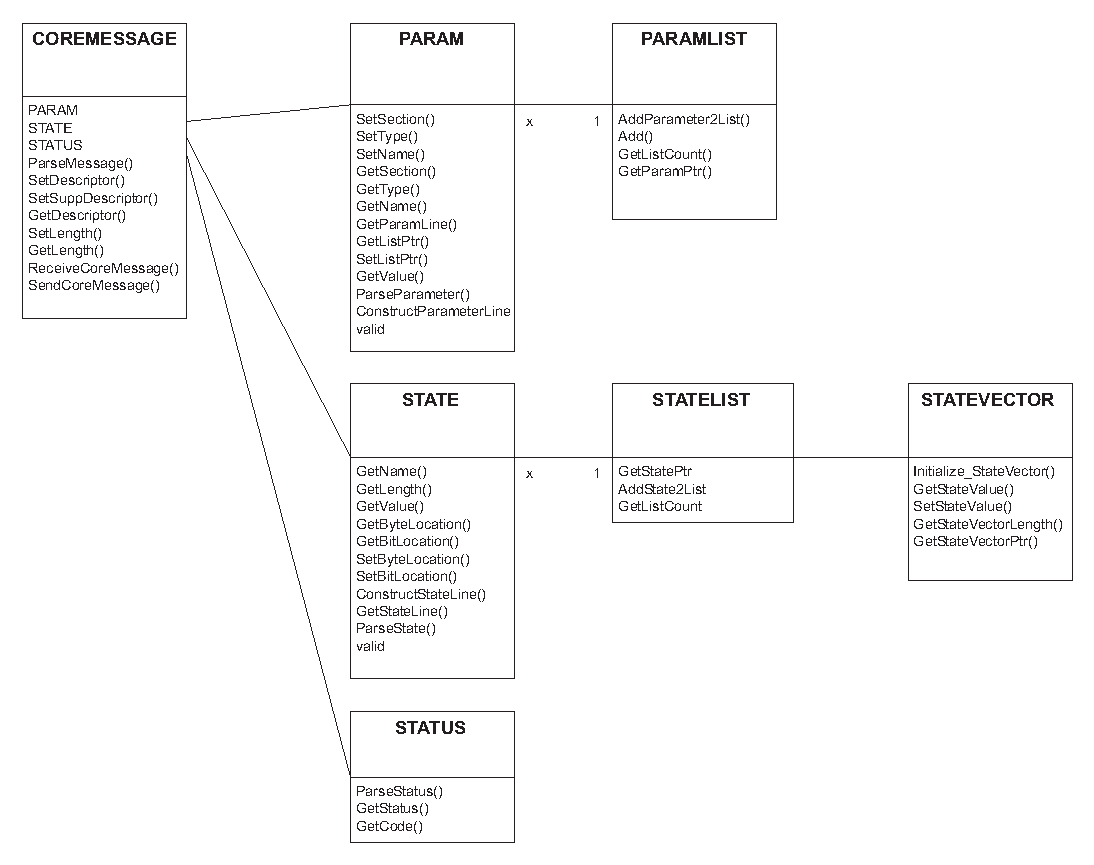
\includegraphics{figures/ERmodel_shells}}}
 \caption{Class model for all shared classes}
\end{figure}


\chapter{Available Filters and their Parameters}
\todo{Not all existing filters are present here.}

\section{EEG Source}
\todo{Documentation for the most important EEG sources?}

\section{Signal Processing}
\subsection{Calibration}

The calibration filter (class \textit{CalibrationFilter}) calibrates the 
incoming EEG signal. It performs a linear scaling, such that each channel is 
expressed in $\mu$V and has a mean of zero (i.e., 
$\mathit{newvalue}=(\mathit{ADvalue}-\mathit{SourceChOffset})*\mathit{SourceChGain}$).

The calibration filter acts only on the subset of channels defined by
\textit{TransmitCh} and \textit{TransmitChList;} regardless of this, the
\textit{SourceChOffset} and \textit{SourceChGain} parameters
refer to the full set of software channels as stored in the data file, in
the order in which they are digitized.

\subsubsection{Requested Parameters}

\begin{table}[ht]
 \centering
 \begin{tabular}{|l|l|l|}
  \hline
  \textbf{Section} & \textbf{Parameter} & \textbf{Data Type}\\
  \hline
  Source & SourceChOffset & floatlist \\
  \hline
  Source & SourceChGain & floatlist \\
  \hline
  Source & AlignChannels & int \\
  \hline
 \end{tabular}
 \caption{Parameters requested by the class CalibrationFilter}
 \todo{Document extension to alignment}
\end{table} 

\textit{SourceChOffset} specifies a list of offsets in AD units -- one value
for each channel. \\
\textit{SourceChGain} specifies a list of gains as used in described formula -- 
one value for each channel. \\
\textit{AlignChannels} specifies whether samples should be aligned in time --
most data acquisition boards multiplex one A/D converter and thus samples
for \textit{SoftwareCh} channels are linearly distributed in time over 
$\frac{1000}{SamplingRate}$ milliseconds (0=no alignment, 1=perform alignment).

\subsubsection{Input/Output}

The input to an instance of this filter class is GenericIntSignal A (dimensions 
\textit{TransmitCh} channels by \textit{SampleBlockSize} elements). Its output 
is Signal B with the same dimensions.


\subsection{Spatial Filter}

The spatial filter class \textit{SpatialFilter} performs for each sample vector 
(\textit{TransmitCh} values -- one for each channel) an operation as shown in 
Figure \ref{spat_filt_op}.

\begin{figure}[ht]
 \centerline{\scalebox{1.0}{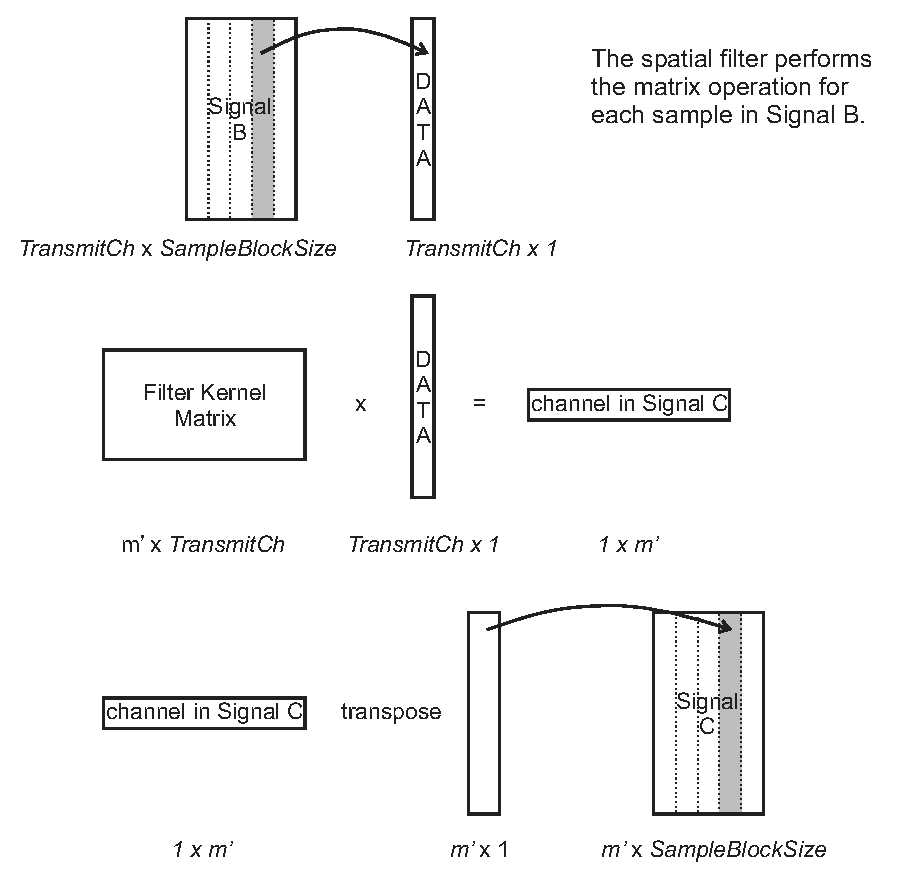
\includegraphics{figures/SpatFiltMatOp}}}
 \caption{Matrix operation on the input signal}
 \label{spat_filt_op}
\end{figure}


\subsubsection{Requested Parameters}

\begin{table}[ht]
 \centering
 \begin{tabular}{|l|l|l|}
  \hline
  \textbf{Section} & \textbf{Parameter} & \textbf{Data Type}\\
  \hline
  Filtering & SpatialFilterKernel & matrix \\
  \hline
 \end{tabular}
 \caption{Parameters requested by the class SpatialFilter}
\end{table} 

The dimensions of \textit{SpatialFilterKernel} are \textit{m'} by 
\textit{TransmitCh}.

\subsubsection{Input/Output}

The input to an instance of this filter class is Signal B (dimensions 
\textit{TransmitCh} channels by \textit{SampleBlockSize} elements). Its output 
is Signal C with the following dimensions: \textit{m'} channels and 
\textit{SampleBlockSize} elements.


\subsection{Temporal Filter Using an AR Model}

Each instance of the temporal filter class \textit{ARFilter} requests 
the following parameters:

\subsubsection{Requested Parameters}

\begin{table}[ht]
 \centering
 \begin{tabular}{|l|l|l|}
  \hline
  \textbf{Section} & \textbf{Parameter} & \textbf{Data Type}\\
  \hline
  Filtering & TempFiltCfg & matrix \\
  \hline
 \end{tabular}
 \caption{Parameters requested by the class ARFilter}
\end{table} 

\textit{TempFiltCfg} is a matrix of dimensionality m' x (max nr. of columns). It
serves to configure the nature of temporal filtering. \\


\subsubsection{Input/Output}

The input to an instance of this filter class is Signal C (dimensions number of 
spatially filtered channels by \textit{SampleBlockSize} elements). Its output is 
Signal D with the following dimensions: m' x n'.



\subsection{Classifier / Translation Algorithm}

An instance of \textit{ClassifierFilter} transforms pre--processed signal 
components into signals that can -- after normalization -- be used for device 
control.

\subsubsection{Requested Parameters}

\begin{table}[ht]
 \centering
 \begin{tabular}{|l|l|l|}
  \hline
  \textbf{Section} & \textbf{Parameter} & \textbf{Data Type}\\
  \hline
  Filtering & MUD & matrix \\
  \hline
  Filtering & MLR & matrix \\
  \hline
 \end{tabular}
 \caption{Parameters requested by the class ClassifierFilter}
\end{table} 

\todo{Fix MUD and MLR description}
\textit{MUD} and \textit{MLR} are matrices of the same dimensionality as Signal 
D (m' x n'). The two scalars in the resulting control signal (Signal E) -- one 
for up/down and one for left/right movement -- each are linear combinations of 
Signal D and their respective weight matrix (\textit{MUD} or \textit{MLR}) as 
follows: $updown=\sum_{i=0,j=0}^{i<m',j<n'}{MUD_{ij}*SignalD_{ij}}$


\subsubsection{Input/Output}

The input to this filter class is Signal D with the following dimensions: m' x 
n'. The output is Signal E with \textit{NumControlSignals} channels and 1 
element per channel.


\subsection{Normalizer}

An instance of \textit{NormalizeFilter} makes each scalar in the vector of
control signals (Signal E) zero mean and thereafter normalizes it to a 
desired range (not exceeding -32767 to +32767).

\subsubsection{Requested Parameters}

\begin{table}[ht]
 \centering
 \begin{tabular}{|l|l|l|}
  \hline
  \textbf{Section} & \textbf{Parameter} & \textbf{Data Type}\\
  \hline
  Filtering & Gain & floatlist \\
  \hline
  Filtering & Intercept & floatlist \\
  \hline
 \end{tabular}
 \caption{Parameters requested by the class NormalizeFilter}
\end{table} 

Each of the \textit{NumControlSignals} scalars in \textit{Gain} and 
\textit{Intercept} are used as follows: 
$SignalF_{i}=Gain_{i}*(SignalE_{i}+Intercept_{i})$


\subsubsection{Input/Output}

The input to this filter class is Signal E with the following dimensions: 
\textit{NumControlSignals} channels and 1 element per channel. Its output,
Signal F, is of the same dimensionality.


\subsection{Slow-Wave-Feedback}

\subsubsection{Author and Introduction}

Description of Signal Processing Module for the Slow-Wave-Feedback written by 
Dr. Thilo Hinterberger, University of T\"ubingen, Germany.

The calculation of the Slow-Wave feedback signal is subdivided into three 
modules: The SW-Filter, which is realized as an efficient boxcar-filter, the 
SetBaseline module, which subtracts a defined baseline from the signal and an 
artifact correction module, which contains two different artifact correction 
modes.  

\begin{figure}[ht]
 \centerline{\scalebox{0.8}{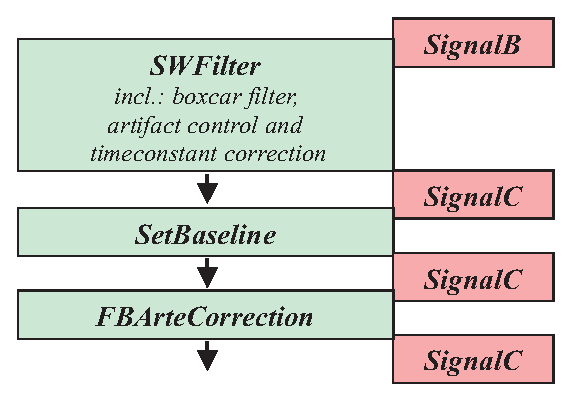
\includegraphics{figures/SWFilterFlow}}}
 \caption{Data flow in the slow wave filter}
 \label{swfilterdataflow}
\end{figure}

\subsubsection{Temporal SW-Filter}

Following states are used:
Artifact (bool) is set to 1 when the signal changes exceed the threshold values defined in ThresholdAmp (see below).  
BeginOfTrial is checked to trigger the start of the trial and reset the internal counter.

\subsubsection{Requested Parameters}

The SW-Filter uses the following parameters:

\begin{verbatim}
SWFilter int SWAvgSpan= 0.5 0.5 0 10 
         // Averaging window in s
SWFilter intlist SWInChList= 3 0 1 2 0 0 63 
         // Channel index of input signal (include artifact channel!)
SWFilter intlist SWOutChList= 3 0 1 2 0 0 63 
         // Channel index of output signal (include artifact channel!)
SWFilter floatlist ThresholdAmp= 3 100 100 400 200 -2000 2000 
         // Threshold for invalid Trial in uV
SWFilter float Tc= 0 16 0 1024 
         // Time constant filter settings in s
Visualize int VisualizeSWFiltering= 1 0 0 1  
          // visualize SW filtered signals (0=no 1=yes)
\end{verbatim}

SWAvgSpan defines the time window of the boxcar-filter. SWInChList defines, 
which channels from Signal B are filtered. They are sorted to the channels in 
Signal C which are selected in SWOutChList. In the Standard setting, three 
channels are filtered. The ThresholdAmp is an artifact control parameter. In 
between one trial (from one BeginOfTrial to the next), the amplitude is not 
allowed to vary more than the in ThresholdAmp defined size in �V. Otherwise the 
trial should be neglected and set as invalid in the application module (state 
Artifact is set to one). A time constant (Tc) correction function simulates a 
real DC-behaviour, even if the amplifier has no DC-option. This can be done by 
the knowledge of the amplifiers' time constant, which is set as the parameter 
Tc. To avoid that the signal will drift towards very high positive or negative 
values, the correction signal is set to zero each time, when BeginOfTrial is 
one. Tc=0 will switch off the Tc-correction. Note: The Tc-correction will only 
work properly, when the A/D-converter and the amplifier puts out 0 when the 
input is 0 �V and there is no electrode polarization! If you are not sure, 
switch off this correction.

\subsubsection{Baseline Setting}

Following states are used:
Baseline (bool) is set to 1 during the baseline period between BaseBegin and BaseEnd. Otherwise it is zero.
BeginOfTrial is checked to trigger the start of the trial and reset the internal counter.

\subsubsection{Requested Parameters}

The SW-Filter uses the following parameters:

\begin{verbatim}
BLFilter float BaseBegin= 0.9 1.9 0 60 
         // Begin of Baseline in s
BLFilter float BaseEnd= 1.0 2.0 0 60 
         // End of Baseline in s
BLFilter intlist BaseChList= 3 1 1 1 1 0 1 
         // 1 to mark that BL is subtracted
Visualize int VisualizeBaselineFiltering= 1 0 0 1  
          // visualize baseline filtered signals (0=no 1=yes)
\end{verbatim}

The baseline is set each trial at the time point BaseEnd seconds after 
BeginOfTrial was set to one. The baseline amplitude is the average amplitude in 
the time interval between BaseBegin and BaseEnd. The baseline is subtracted of 
all channels marked with 1 in the BaseChList. As default, baseline subtraction 
is applied on all three channels.

This version still uses the parameters BIPts and FIPts, which define the 
duration of the baseline-interval and the feedback-interval in seconds. These 
parameters are used for the buffer, which needs the duration of a trial. They 
will be no longer used in the next version.  

\subsubsection{Artifact Correction}

Following states are used:

Artifact (bool) is set to 1 only in ArteMode=3 when the feedback signal is set 
to zero due to the EOG artifact BeginOfTrial is checked to trigger the start of 
the trial and reset the internal counter.

\subsubsection{Requested Parameters}

The SW-Filter uses the following parameters:

\begin{verbatim}
ArteFilter intlist ArteChList= 3 2 2 -1 2 -1 63
  // Assignment of artefact channels, -1: no artifact channel
ArteFilter floatlist ArteFactorList= 7 0.15 0.15 0 0 0 0 0 0 -1 1
  // Influence of artefact channel on input channel,
     -1: no artifact channel
ArteFilter int ArteMode= 0 1 0 3
  // Artefact correction mode, 0 off, 1 continuous, 2 conditioned
Visualize int VisualizeFBArteCorFiltering= 1 0 0 1 
  // visualize FBArte corrected signals (0=no 1=yes)
\end{verbatim}

Artifacts are corrected on all channels which are not marked with -1
in the ArteChList. For the correction, the channel number at the
position of the channel in the ArteChList is used as artifact channel.
For example, the standard setting corrects the channels 0 and 1 by using
channel 2 for the correction. The correction factor is the factor set
in ArteFactorList, 0.15 in the standard setting.

For the ArteMode parameter, the following values are possible: 
\begin{itemize}
 \item\verb|ArteMode 0| switches this filter off.
 \item\verb|ArteMode 1| will subtract the artifact channel multiplied 
      with a constant factor.
 \item\verb|ArteMode 2| will correct the signal according to Koutchoubey, 1997:
      If the artifact signal has the same sign as the control signal, a correction
      is applied by subtracting the artifact signal; otherwise, no correction 
      is performed. If the artifact crosses a threshold value, feedback is
      suppressed.
 \item\verb|ArteMode 3| is working identically to \verb|ArteMode 2| but sets the
      Artifact state to 1 when the feedback is set to zero.
\end{itemize}

\section{Application}
\todo{Documentation for the most important Application modules?}
\subsection{Right Justified Boxes Task}
\label{section_rjb_task}

The right justified box task is a cursor task, in which the subject tries to hit 
one out of \textit{n} targets on a screen in trials of equal length. As listed 
in 
figure \ref{rjb_task}, the task requests and 
controls specific states.

Whatever signal processing algorithm is used, it can passively monitor these 
states and modify its operation accordingly, e.g., one algorithm might derive 
its baseline from the inter-trial interval (i.e., ITI), whereas another might 
calculate it differently. In this fashion, signal processing algorithms can be 
interchanged without affecting the user application.

\begin{figure}[ht]
 \centerline{\scalebox{0.6}{\includegraphics{figures/RJBtask}}}
 \caption{Time Line for Right Justified Box task. The top-most target position
          corresponds to TargetCode=1. TargetCode increases towards the bottom.
          ResultCode corresponds to the target actually selected. Thus, if
          TargetCode equals ResultCode, the trial was a hit, otherwise a miss.}
 \label{rjb_task}
\end{figure}

Figure \ref{rjb_task} illustrates the time line for the right justified box task 
and, for each time interval, its respective content for each state. 

1 is the intertrial interval, were the screen is blank and baseline data can be 
collected (optional). In 2 the target is presented, but the cursor is absent (no 
feedback).  In 3 the cursor is present and it's vertical movement is controlled 
by the user's EEG.  Horizontal cursor movement is under computer control and is 
at a constant rate.  In 4 the cursor approaches the target and in 5 the target 
has been hit and trial-outcome feedback is presented.  In 6 the screen is blank 
(intertrial interval again) and in 7 another target is presented.


%Most components described in the System Architecture section will require a more 
%detailed discussion. Other lower-level components and subcomponents may need to 
%be described as well. Each subsection of this section will refer to or contain a 
%detailed description of a system software component. The discussion provided 
%should cover the following software component attributes: 

%Classification 

%The kind of component, such as a subsystem, module, class, package, function, 
%file, etc. .... 

%Definition 

%The specific purpose and semantic meaning of the component. This may need to 
%refer back to the requirements specification. 

%Responsibilities 

%The primary responsibilities and/or behavior of this component. What does this 
%component accomplish? What roles does it play? What kinds of services does it 
%provide to its clients? For some components, this may need to refer back to the 
%requirements specification. 

%Constraints 

%Any relevant assumptions, limitations, or constraints for this component. This 
%should include constraints on timing, storage, or component state, and might 
%include rules for interacting with this component (encompassing preconditions, 
%postconditions, invariants, other constraints on input or output values and 
%local or global values, data formats and data access, synchronization, 
%exceptions, etc.) 


%Composition 

%A description of the use and meaning of the subcomponents that are a part of 
%this component. 


%Uses/Interactions 

%A description of this components collaborations with other components. What 
%other components is this entity used by? What other components does this entity 
%use (this would include any side-effects this entity might have on other parts 
%of the system)? This concerns the method of interaction as well as the 
%interaction itself. Object-oriented designs should include a description of any 
%known or anticipated subclasses, superclasses, and metaclasses. 

%Resources 

%A description of any and all resources that are managed, affected, or needed by 
%this entity. Resources are entities external to the design such as memory, 
%processors, printers, databases, or a software library. This should include a 
%discussion of any possible race conditions and/or deadlock situations, and how 
%they might be resolved. 


%Processing 

%A description of precisely how this components goes about performing the duties 
%necessary to fulfill its responsibilities. This should encompass a description 
%of any algorithms used; changes of state; relevant time or space complexity; 
%concurrency; methods of creation, initialization, and cleanup; and handling of 
%exceptional conditions. 

%Interface/Exports 

%The set of services (resources, data, types, constants, subroutines, and 
%exceptions) that are provided by this component. The precise definition or 
%declaration of each such element should be present, along with comments or 
%annotations describing the meanings of values, parameters, etc. .... For each 
%service element described, include (or provide a reference) in its discussion a 
%description of its important software component attributes (Classification, 
%Definition, Responsibilities, Constraints, Composition, Uses, Resources, 
%Processing, and Interface). 

%Much of the information that appears in this section is not necessarily expected 
%to be kept separate from the source code. In fact, much of the information can 
%be gleaned from the source itself (especially if it is adequately commented). 
%This section should not copy or reproduce information that can be easily 
%obtained from reading the source code (this would be an unwanted and unnecessary 
%duplication of effort and would be very difficult to keep up-to-date). It is 
%recommended that most of this information be contained in the source (with 
%appropriate comments for each component, subsystem, module, and subroutine). 
%Hence, it is expected that this section will largely consist of references to or 
%excerpts of annotated diagrams and source code. Any referenced diagrams or 
%source code excerpts should be provided at any design reviews. 